\documentclass[aspectratio=169]{beamer}
\usetheme{Berlin}
\usepackage[brazilian]{babel}
\usepackage[utf8]{inputenc}
\usepackage{graphicx}
\graphicspath{{img/}}
\usepackage{amsmath,amsfonts,amssymb}
\setbeamercovered{transparent}
\usepackage{multimedia}

\title{Inserir vídeo, áudio e transição}
\subtitle{Curso de BEAMER}
\author[César]{César A. de Magalhães}
\institute[UNOPAR]{Universidade do Norte do Paraná \\ https://vestibular.unoparead.com.br}
\date{\today}
\logo{
\includegraphics[scale=0.25]{ctan-leao.jpg}}

\begin{document}
	\begin{frame}
		\titlepage
	\end{frame}
	\begin{frame}{Aquarela: Toquinho}
		\begin{center}
			\movie[externalviewer]{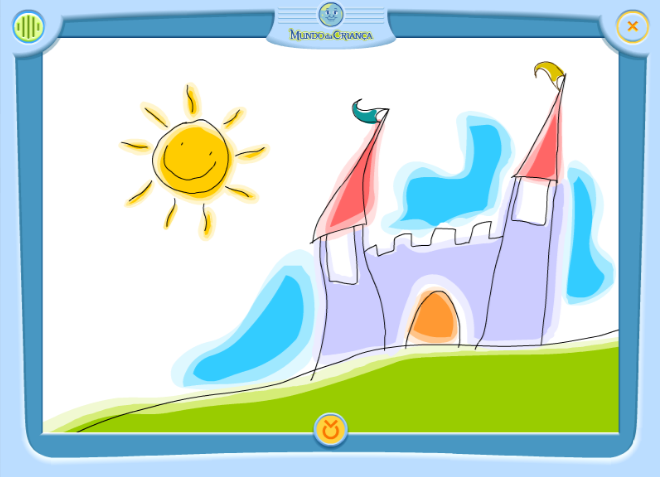
\includegraphics[scale=0.2]{aquarela.png}}{media/aquarela.mp4}
		\end{center}		
	\end{frame}	
	\begin{frame}{Efeito sonoro}
		\sound[externalviewer]{Car Door Ajar Beep}{media/beep.mp3}
	\end{frame}
		
	\newcount{\nomedocontador}
	\newdimen{\nomedadimensao}
	\begin{frame}{Título do terceiro quadro}
		\animatevalue<1-7>{\nomedocontador}{0}{100}
		\animatevalue<1-7>{\nomedadimensao}{0cm}{4cm}
		
		\textcolor{red!\the\nomedocontador!blue}{Aqui vem outro texto.}
		\hspace{\nomedadimensao} Aqui vem o texto.
		
		\animate<2-5>
		\begin{itemize}[<+->]
			\item Slide 3.1
			\item Slide 3.2
			\item Slide 3.3
			\item Slide 3.4
			\item Slide 3.5
			\item Slide 3.5
			\item Slide 3.7
		\end{itemize}
	\end{frame}
	
	\begin{frame}{Título do quarto quadro}
		
		\transdissolve[duration=2]<2>
		\transblindshorizontal[duration=2]<3>
		\transblindsvertical[duration=2]<4>
		\transboxin[duration=2]<5>
		\transglitter[duration=2, direction=90]<6>
		\transsplithorizontalin[duration=2]<7>
		
		\begin{itemize}[<+->]
			\item Slide 4.1
			\item Slide 4.2
			\item Slide 4.3
			\item Slide 4.4
			\item Slide 4.5
			\item Slide 4.5
			\item Slide 4.7
		\end{itemize}
	\end{frame}
\end{document}